\begin{center}
	\textbf{\LARGE{Metoda končnih elementov, ki minimizira kvadrat ostanka aproksimacije (\texttt{LSFEM})}}\\[0.25cm]
	\large{Seminarska naloga pri Naprednih numeričnih metodah}\\[0.7cm]
\end{center}

Numerično reševanje parcialnih diferencialnih enačb (\texttt{PDE}) je zaradi pomanjkanja vsestranskega algoritma še zmeraj bolj umetnost kot ustaljena znanost \cite{JiangB-LSFEM}. Pri zapletenih problemih hitro prispemo do vznožja gore matematične teorije, ki je ni moč zaobiti. Zaradi množice različnih pristopov reševanja ter raztresene in neprijazno napisane literature, lahko le ugibamo, kako visoko se bomo na poti do prelaza morali povzpeti. Zapletenim problemom prostorske dinamike v:
\begin{center}
	\begin{tabular}[h]{lll}
		\tabitem dinamiki tekočin,\hspace{1cm}	&	\tabitem termodinamiki,\hspace{2.5cm}	&	\tabitem elektrodinamiki,\\
		\tabitem kvantni teoriji,	&	\tabitem splošni teoriji relativnosti,&	\\
	\end{tabular}
\end{center}
kjer naletimo na \texttt{PDE}, se tako tudi v višjem izobraževanju najraje izognemo. Metoda končnih elementov (\texttt{FEM}), ki minimizira kvadrat ostanka aproksimacije (\texttt{LSFEM} = Least Squares \texttt{FEM}), obeta razvoj vsestranskega algoritma za reševanje \texttt{PDE} in s tem približanje omenjenih problemov širšemu krogu raziskovalcev.

\section{Temelji \texttt{LSFEM}}
Kadar obravnavamo prostorsko dinamiko (npr.\ prevajanje toplote ali tok tekočine), lahko fizični prostor modeliramo kot 1, 2 ali 3-mnogoterost. Temelje \texttt{LSFEM} bomo polagali na splošnem primeru $d$-mnogoterosti, v prid predstavljivosti pa na njih sproti gradili konkretni 2D primer.\\[-0.1cm]
\begin{wrapfigure}{r}{5.5cm}
	\centering
	\captionsetup{type=figure}
	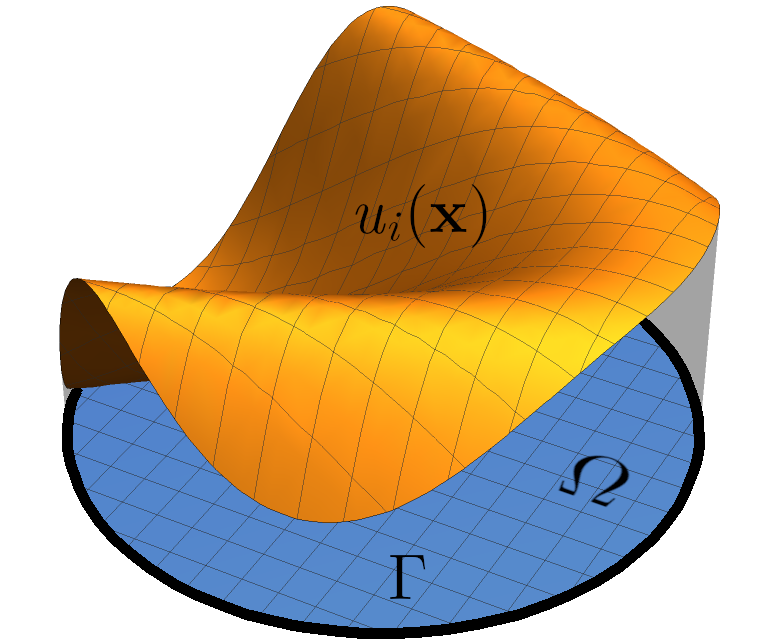
\includegraphics[width=5.5cm]{Slike/funkcijaInDomenaG}
	\caption{Domena $\Omega$, meja domene $\Gamma$ in komponenta rešitve $u_i(\mathbf{x})$.}
\label{fig:funkInDom}
\vspace{-2.4cm}
\end{wrapfigure}
Naj bo torej prizorišče dogajanja $d$-mnogoterost $\Omega$, opremljena s krajevnim vektorjem $\mathbf{x} = \{x_1, ..., x_d\}$. Pri reševanju sistema $m$ \texttt{PDE} iščemo nabor funkcij $\mathbf{u}(\mathbf{x}) =  \{u_1(\mathbf{x}), ..., u_m(\mathbf{x})\}$, ki v vsaki točki domene $\Omega$ zadosti sistemu \texttt{PDE}, na meji $\Gamma$ pa robnim pogojem (slika \ref{fig:funkInDom}). Za primer vzemimo stacionarne Stokesove enačbe v 2D:\\[0.1cm]
\begin{minipage}{5.0cm}
\begin{IEEEeqnarray}{rl}
	\frac{\pd u}{\pd x} + \frac{\pd v}{\pd y} &= 0 \ , \\[0.2cm]
	\frac{\pd p}{\pd x} + \frac{\pd \omega}{\pd y} &= f_1 \ ,
\end{IEEEeqnarray}
\end{minipage}
\begin{minipage}{5.3cm}
\begin{IEEEeqnarray}{rl}
	\frac{\pd p}{\pd y} - \frac{\pd \omega}{\pd x} &= f_2 \ , \\[0.2cm]
	\omega - \frac{\pd u}{\pd y} - \frac{\pd v}{\pd x} &= 0 \ .
\end{IEEEeqnarray}
\end{minipage}\\[0.4cm]
Stokesove enačbe so poenostavitev nelinearnih Navier-Stokesovih enačb. Opisujejo

Pri \texttt{FEM} ne operiramo neposredno na \texttt{PDE}, ampak jih najprej pretvorimo v enakovreden variacijski problem. Za poljubno funkcijo $\mathbf{w}(\mathbf{x})$ zapišemo funkcional $I[\mathbf{w}(\mathbf{x})]$, ki  zavzame minimalno vrednost, kadar je $\mathbf{w}$ enaka rešitvi. Ta funkcional je pri vseh različicah \texttt{FEM} integral neke funkcije $F = F\left(\mathbf{w}\right)$ po domeni $\Omega$:
\begin{equation}
	I[\mathbf{w}(\mathbf{x})] = \int_{\Omega} F\left(\mathbf{w}(\mathbf{x})\right) \, \ud \Omega \hspace{1.1cm} \texttt{funkcional} \quad .
\end{equation}
Kot vemo, poiščemo minimum funkcionala $I$ tako, da za $\mathbf{w}$ vstavimo:

\setlength{\textheight}{26.5cm}			% Header Lower Margin to
\pagebreak
\setlength{\topmargin}{1.6cm}			% Header Top Margin Height
\setlength{\headheight}{0.0cm}
\setlength{\headsep}{0.0cm}			% Header Lower Margin Height	 Footer height
\fancyhf{}
\fancyfoot[C]{\thepage}
\begin{equation}
	\mathbf{w}(\mathbf{x}, \varepsilon) = \mathbf{u}(\mathbf{x}) + \varepsilon \mathbf{v}(\mathbf{x}) \quad ,
\end{equation}
kjer je $\mathbf{v}(\mathbf{x})$ poljuben odmik od rešitve $\mathbf{u}(\mathbf{x})$, $\varepsilon$ pa skalar. Odvajamo po $\varepsilon$ in odvod enačimo z 0:
\begin{equation}
\frac{\ud I}{\ud \varepsilon} = \int_{\Omega} \frac{\ud}{\ud \varepsilon} F(\mathbf{w}) \, \ud \Omega = \int_{\Omega} \frac{\ud F}{\ud \mathbf{w}} \cdot \frac{\ud \mathbf{w}}{\ud \varepsilon} \ \ud \Omega = \int_{\Omega} \frac{\ud F}{\ud \mathbf{w}} \cdot \mathbf{v} \ \ud \Omega = 0 \hspace{0.9cm} \texttt{prva variacija} \ .
\end{equation}

Fizikalno najintuitivnejša je \textbf{Rayleigh-Ritzeva različica}, kjer za $F$ uporabimo energijski potencial sistema \texttt{PDE}. Rešitev $\mathbf{u}(\mathbf{x})$ je potemtakem funkcija, ki minimizira totalno potencialno energijo sistema. Rayleigh-Ritzeva različica poseduje lastnost najboljšega približka (minimizira razliko energijskih norm numerične in eksaktne rešitve), hkrati pa vodi do sistema linearnih algebrajskih enačb, ki je zelo prikladen za reševanje s hitrimi iteracijskimi metodami.

Z Rayleigh-Ritzevo metodo dobimo sistem linearnih algebrajskih enačb za 

Galerkin, Najmanših kvadratov \cite{JiangB-LSFEM}
Basic lemma of variational principles: Temeljni lema variacijskih načel.